\chapter{Deseño}

Neste capítulo descríbese como se constrúe o sistema: a súa arquitectura xeral, a
división en compoñentes e a comunicación entre eles, o modelo de datos, o deseño da API
e dos extremos cliente e servidor, os fluxos máis relevantes e, por último, o
equipamento hardware e software empregado. Sempre que é posible recórrese a
representacións gráficas para facilitar a comprensión da estrutura do produto.

\section{Arquitectura xeral do sistema}

Telaria segue unha arquitectura \textbf{cliente–servidor} de tres capas lóxicas
(presentación, lóxica de negocio e persistencia) e adopta un enfoque \textit{API-first}:
o contrato da API, especificado con OpenAPI, é o punto de partida do desenvolvemento e o
elemento que vincula o cliente co servidor. A Figura~\ref{fig:arquitectura} mostra a
visión de conxunto.

\begin{figure}[H]
  \centering
  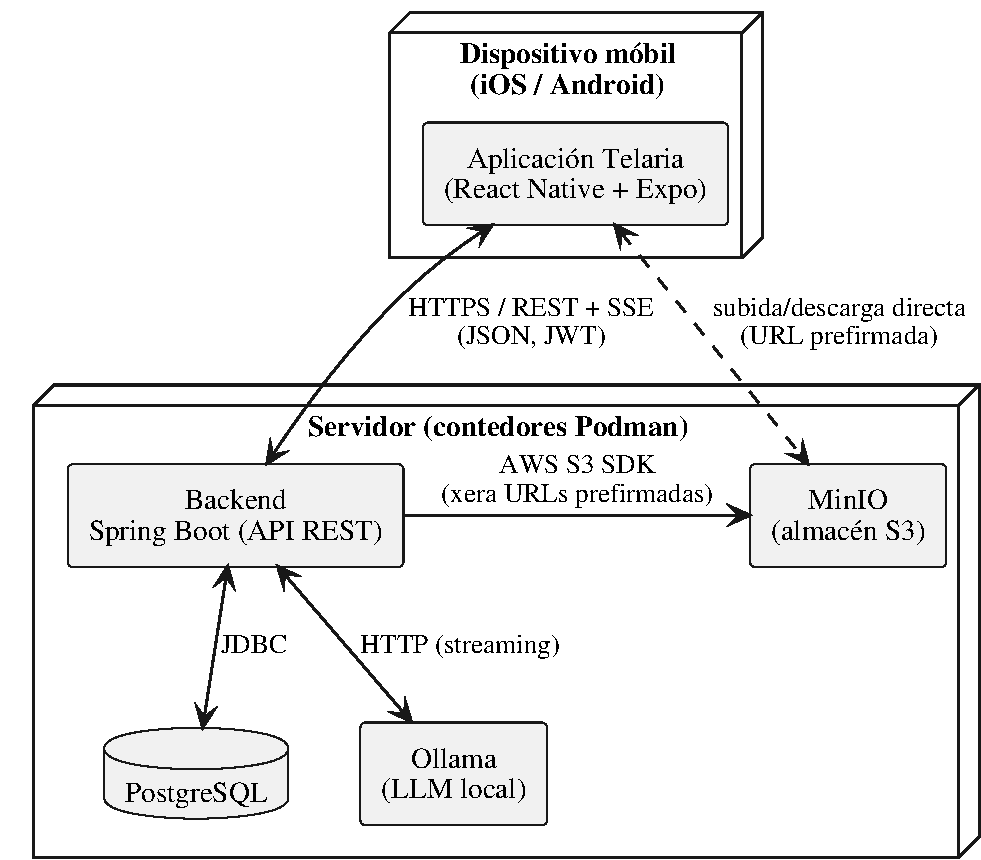
\includegraphics[width=0.72\textwidth]{diagrams/arquitectura.pdf}
  \caption{Arquitectura xeral e despregamento de Telaria.}
  \label{fig:arquitectura}
\end{figure}

O \textbf{cliente} é unha aplicación móbil multiplataforma (React Native + Expo) que se
executa en iOS e Android. O \textbf{servidor} agrupa, en contedores xestionados con
Podman, o backend Spring Boot e os tres servizos de apoio: a base de datos PostgreSQL, o
almacén de obxectos compatible con S3 (MinIO) e o motor de inferencia de modelos de
linguaxe (Ollama).

A comunicación principal entre cliente e servidor realízase sobre HTTP mediante unha API
REST que intercambia JSON e protexe cada petición cun \textit{access token} JWT. Para as
funcionalidades en tempo real (chat de grupo e asistente de IA), o servidor emprega
\textit{Server-Sent Events} (SSE), que permiten un fluxo unidireccional de eventos do
servidor cara ao cliente sobre a mesma conexión HTTP. Finalmente, a subida e a descarga
de documentos non pasan polo backend: este limítase a xerar \textit{URLs prefirmadas} co
que o cliente fala \textbf{directamente} co almacén de obxectos, descargando o servidor
da transferencia de ficheiros.

\section{Arquitectura do backend}

O backend organízase nunha arquitectura por capas que separa claramente as
responsabilidades, como se aprecia na Figura~\ref{fig:backend}.

\begin{figure}[H]
  \centering
  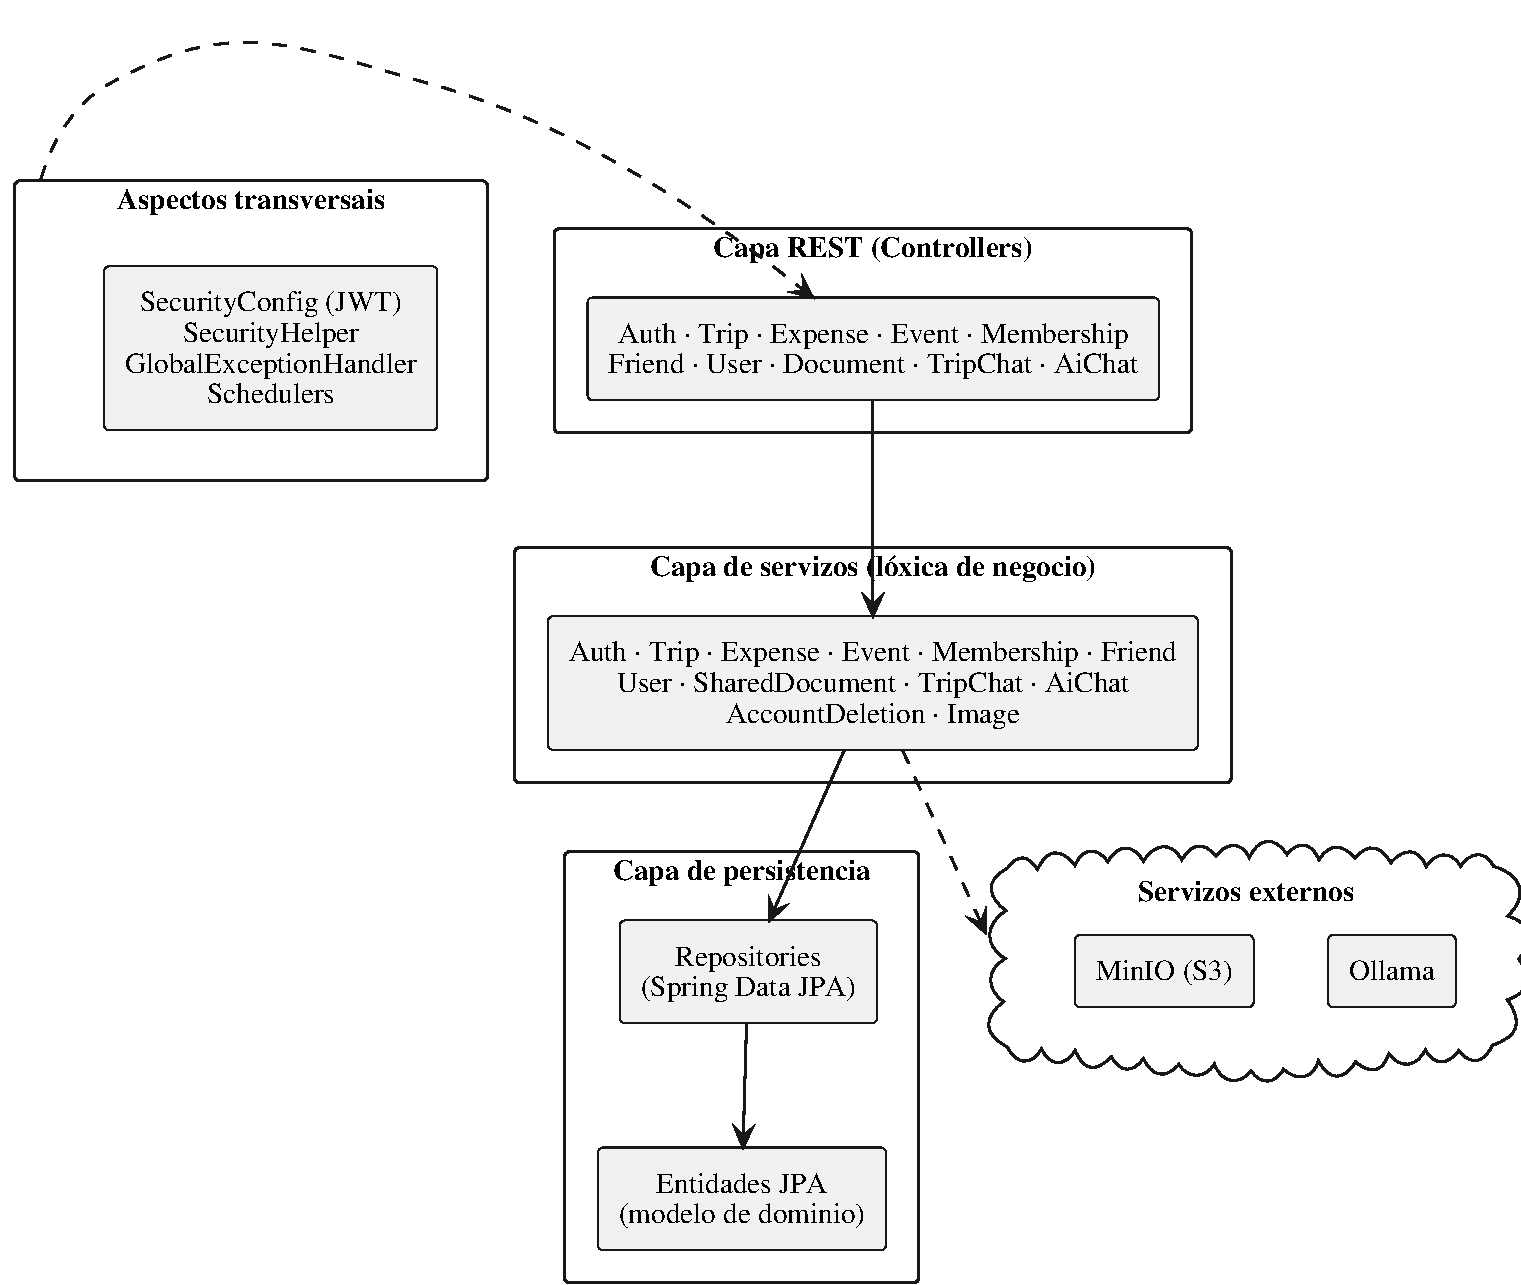
\includegraphics[width=0.85\textwidth]{diagrams/backend-componentes.pdf}
  \caption{Compoñentes e capas do backend.}
  \label{fig:backend}
\end{figure}

\begin{itemize}
  \item \textbf{Capa REST (controllers).} Expón os \textit{endpoints} da API. As
        interfaces destes controladores xéranse automaticamente a partir do contrato
        OpenAPI, e as clases que as implementan conteñen unicamente a tradución entre a
        petición HTTP e a chamada ao servizo correspondente.
  \item \textbf{Capa de servizos.} Concentra a lóxica de negocio: validacións,
        cálculo de liquidacións, resolución de invitacións e solicitudes, xestión de
        ficheiros, etc. É a única capa que coordina varias entidades e repositorios
        dentro dunha mesma transacción.
  \item \textbf{Capa de persistencia.} Componse dos repositorios de Spring Data JPA e
        das entidades do modelo de dominio, que Hibernate mapea ás táboas de PostgreSQL.
  \item \textbf{Aspectos transversais.} A configuración de seguridade (validación de
        tokens JWT con Spring Security), a utilidade de extracción do usuario autenticado
        (\texttt{SecurityHelper}), o manexo centralizado de erros
        (\texttt{GlobalExceptionHandler}, que devolve respostas no formato
        \textit{Problem Details}, RFC~7807)~\cite{rfc7807} e as tarefas programadas
        (\textit{schedulers}) de limpeza e xeración de miniaturas.
\end{itemize}

A autorización aplícase na capa de servizos: o acceso aos datos dunha viaxe verifícase
comprobando que o usuario autenticado pertence aos seus membros, de modo que ningún
usuario poida acceder á información de viaxes das que non forma parte.

\section{Modelo de datos}

A Figura~\ref{fig:modelo} representa o modelo de dominio coas entidades persistentes e as
súas relacións.

\begin{figure}[H]
  \centering
  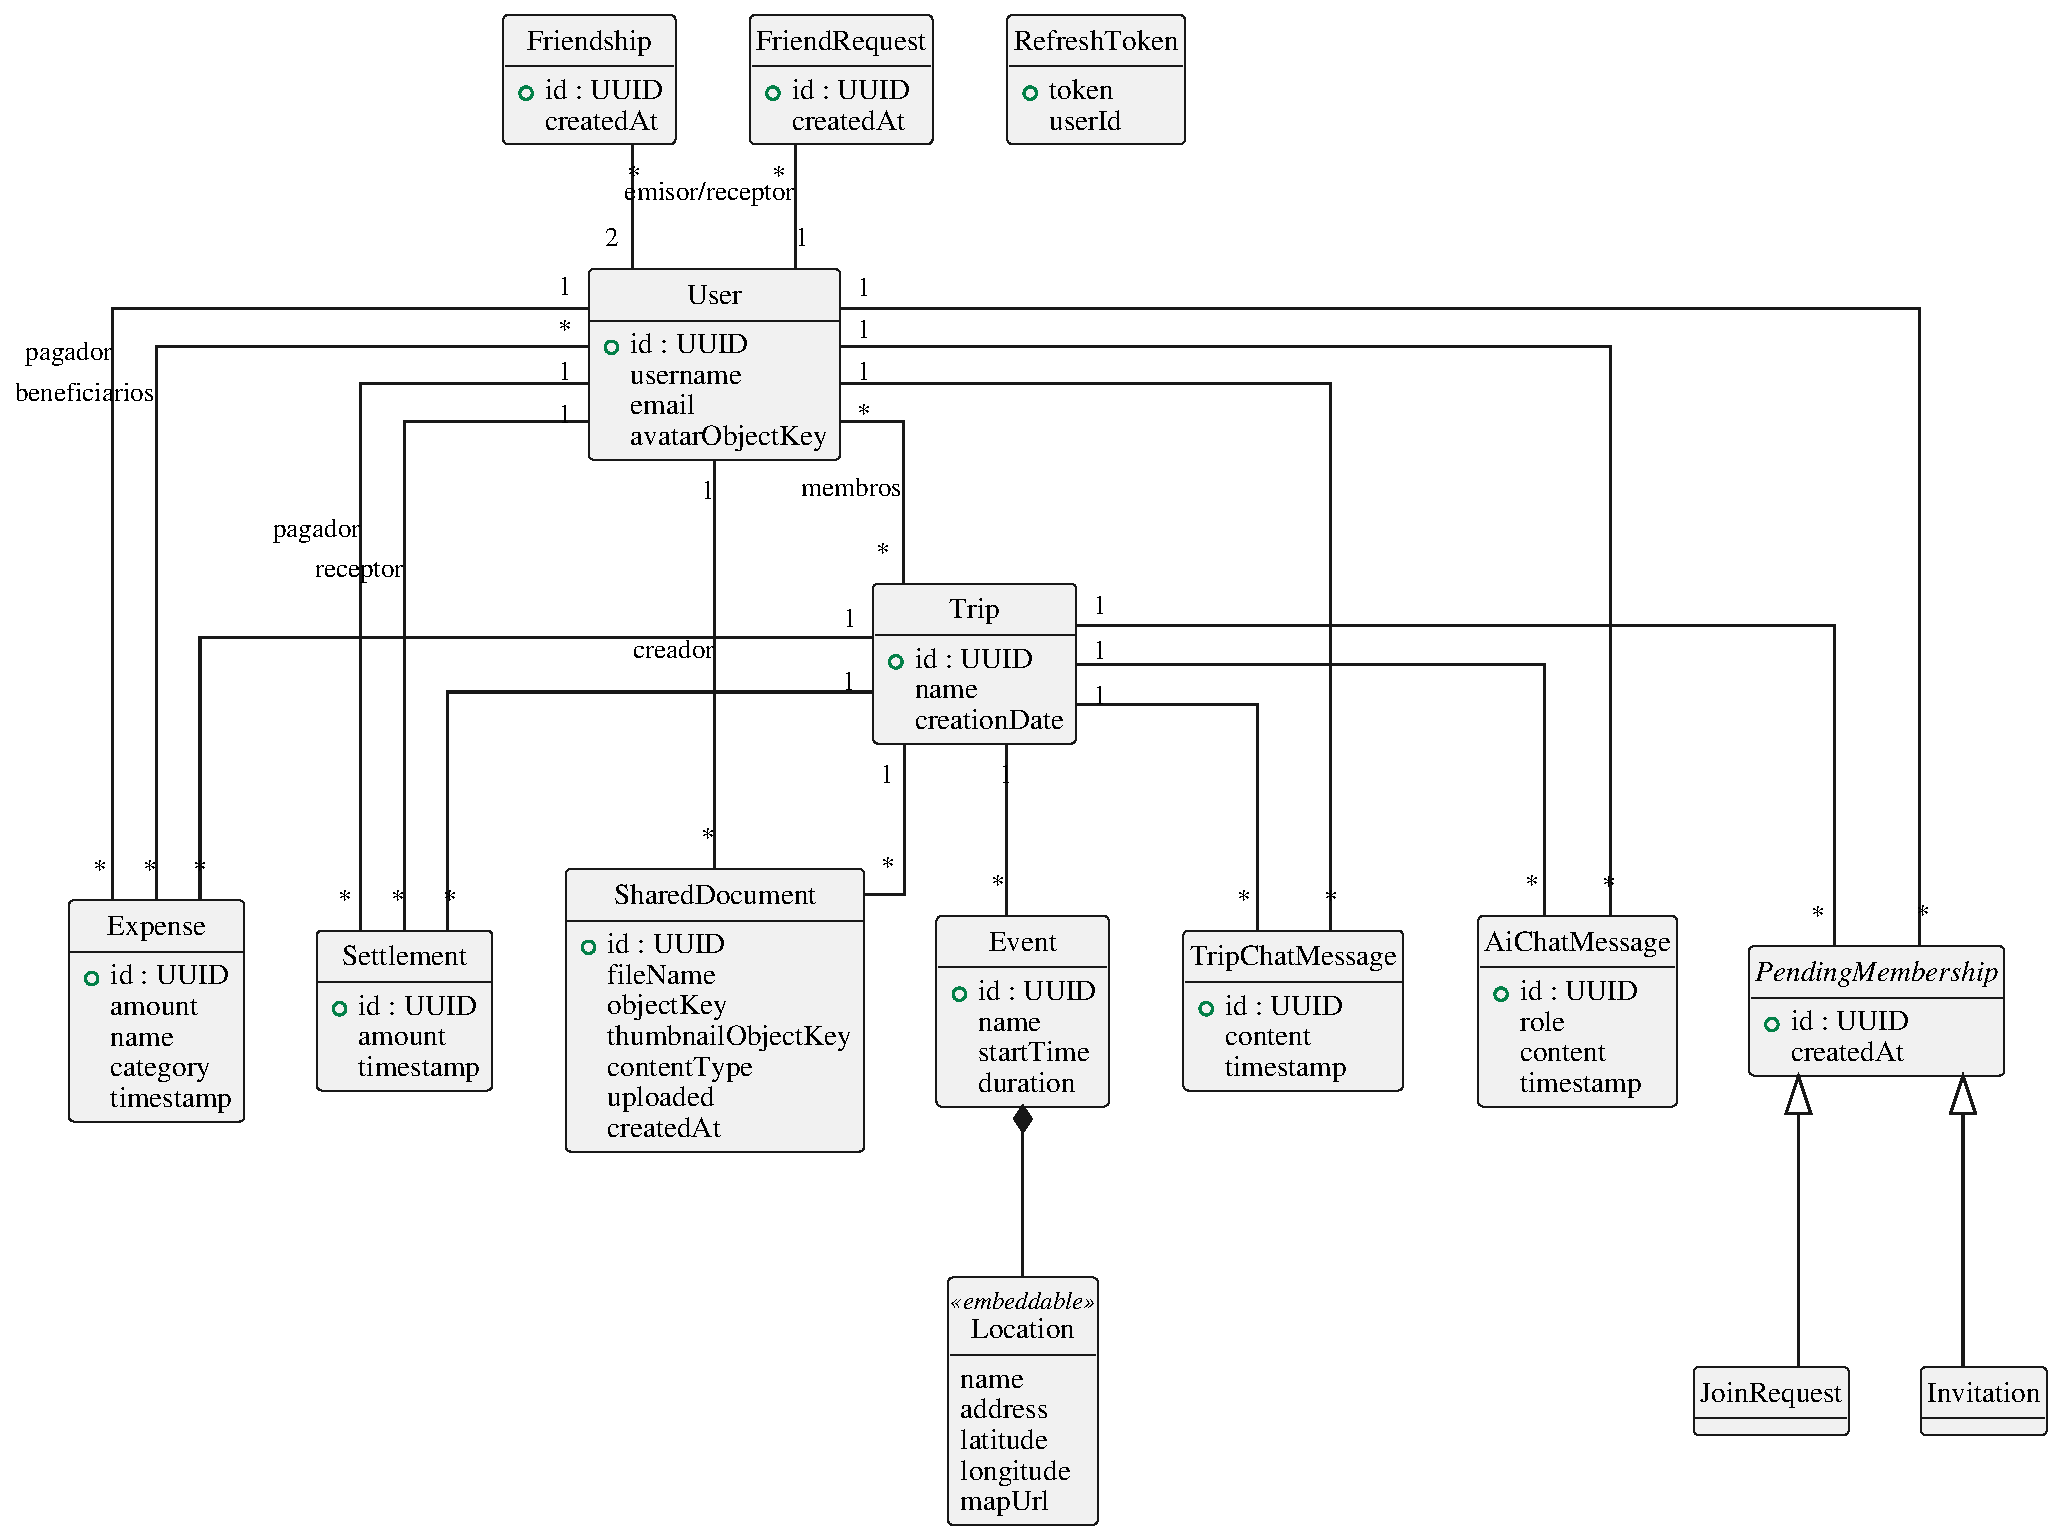
\includegraphics[width=\textwidth]{diagrams/modelo-datos.pdf}
  \caption{Modelo de datos (entidades e relacións principais).}
  \label{fig:modelo}
\end{figure}

As decisións de deseño máis salientables son:

\begin{itemize}
  \item \textbf{Identificadores UUID.} Todas as entidades principais empregan UUID como
        clave primaria, o que evita expor identificadores secuenciais e facilita a
        xeración de claves no lado da aplicación.
  \item \textbf{Relacións varios-a-varios.} A pertenza ás viaxes
        (\texttt{User}\,--\,\texttt{Trip}) e os beneficiarios dun gasto
        (\texttt{Expense}\,--\,\texttt{User}) modélanse mediante táboas de unión.
  \item \textbf{Normalización das amizades.} Cada \texttt{Friendship} almacena os dous
        usuarios de forma ordenada (o de identificador menor primeiro), o que garante a
        unicidade da parella e simplifica as consultas bidireccionais.
  \item \textbf{Valor embebido.} A localización dun evento (\texttt{Location}: nome,
        enderezo, coordenadas e URL de mapa) modélase como un obxecto embebido dentro de
        \texttt{Event}, ao non ter identidade propia (considérase que os diferentes eventos
         non compartirán ubicación frecuentemente).
  \item \textbf{Xerarquía de membros pendentes.} \texttt{Invitation} e
        \texttt{JoinRequest} comparten estrutura (viaxe, usuario e marca temporal) a
        través da superclase \texttt{PendingMembership}, diferenciándose só na
        dirección da petición.
  \item \textbf{Token de refresco persistente.} O \texttt{RefreshToken} almacénase no
        servidor para poder invalidalo no peche de sesión.
\end{itemize}

O esquema da base de datos non se xestiona con ferramentas de migración: emprégase a
xeración automática de Hibernate (\texttt{ddl-auto}), apropiada para o contexto deste
proxecto. Na sección de conclusións recóllese a adopción de migracións explícitas como
posible mellora de cara a un entorno de produción.

\section{Deseño da API REST}

A API é o contrato central do sistema e especifícase con \textbf{OpenAPI} de forma
modular: un documento principal (\texttt{api.yaml}) referencia, mediante \texttt{\$ref},
ficheiros independentes para as rutas (\texttt{paths/}) e para os esquemas de datos
(\texttt{schemas/}). Esta organización mantén o contrato lexible malia o seu tamaño.

A partir deste contrato xérase código automaticamente en ambos os extremos:

\begin{itemize}
  \item No \textbf{backend}, o complemento \textit{OpenAPI Generator} produce as
        interfaces dos controladores e os obxectos de transferencia de datos (DTO).
  \item No \textbf{frontend}, a ferramenta \texttt{openapi-typescript} xera os tipos
        TypeScript que describen as peticións e respostas.
\end{itemize}

Deste xeito, calquera cambio no contrato propágase automaticamente como tipos a ambos os
extremos, e calquera incoherencia detéctase en tempo de compilación. Ademais, a partir
da mesma especificación ofrécese documentación interactiva da API (Swagger UI). A
Táboa~\ref{tab:recursos} resume os principais recursos da API.

\begin{table}[H]
  \centering
  \begin{tabularx}{\textwidth}{@{}lX@{}}
    \toprule
    \textbf{Recurso} & \textbf{Responsabilidade} \\
    \midrule
    \texttt{/auth}                    & Rexistro, inicio e peche de sesión, renovación de tokens. \\
    \texttt{/users}                   & Perfil, contrasinal, avatar, eliminación de conta. \\
    \texttt{/trips}                   & Creación e consulta de viaxes. \\
    \texttt{/trips/[tripID]/expenses}      & Gastos, balances e liquidacións. \\
    \texttt{/trips/[tripID]/events}        & Eventos do calendario. \\
    \texttt{/trips/[tripID]/documents}     & Documentos compartidos (subida en varios pasos). \\
    \texttt{/trips/[tripID]/group-chat}    & Chat de grupo (consulta, envío e fluxo SSE). \\
    \texttt{/trips/[tripID]/ai-chat}       & Asistente de IA (historial e resposta en \textit{streaming}). \\
    Invitacións, solicitudes, amizades & Xestión de membros e da rede social de usuarios. \\
    \bottomrule
  \end{tabularx}
  \caption{Resumo dos principais recursos da API REST.}
  \label{tab:recursos}
\end{table}

\section{Arquitectura do frontend}

O cliente organízase tamén por capas, como amosa a
Figura~\ref{fig:frontend}. A navegación baséase en \textbf{Expo Router}, un sistema de
rutas baseado na estrutura de ficheiros, que agrupa as pantallas en tres grupos
(\texttt{(auth)}, \texttt{(main)} e \texttt{(trip)}).

\begin{figure}[H]
  \centering
  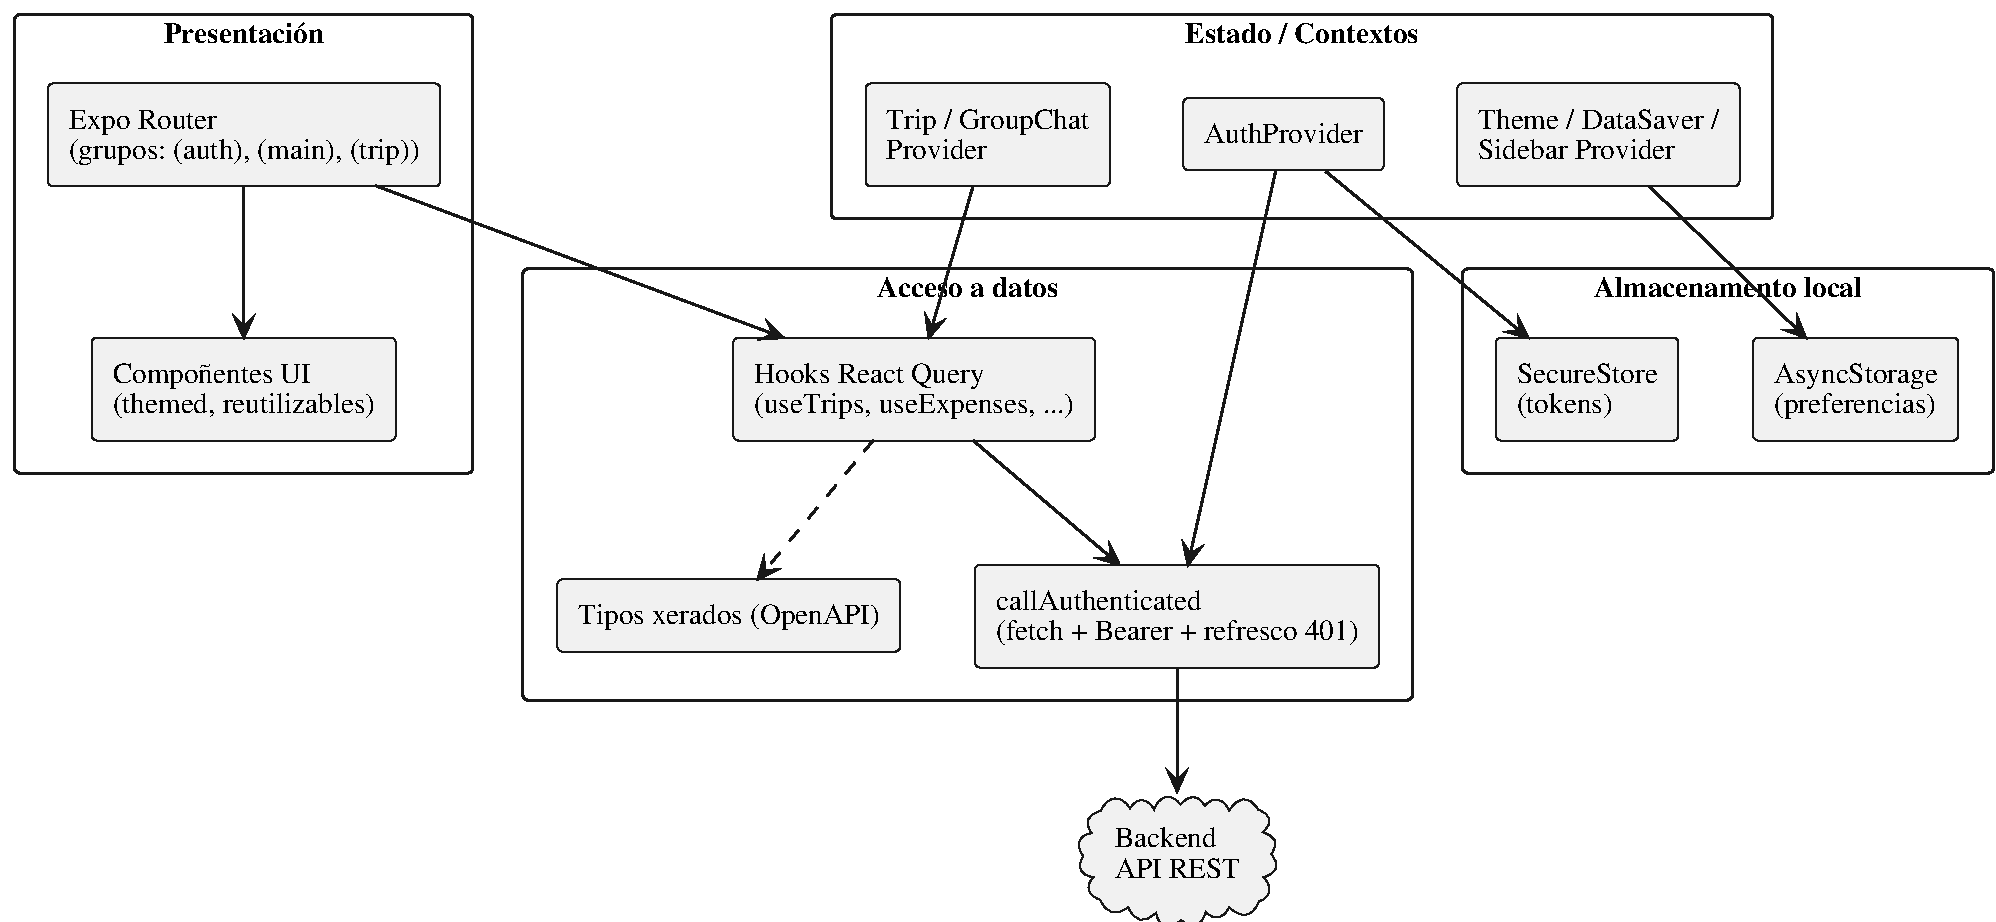
\includegraphics[width=\textwidth]{diagrams/frontend-arquitectura.pdf}
  \caption{Arquitectura do frontend.}
  \label{fig:frontend}
\end{figure}

O estado da aplicación divídese en dous tipos. O \textbf{estado de servidor} (datos que
proveñen do backend) xestiónase con \textbf{React Query}~\cite{reactquery}, que se encarga da caché, da
revalidación e da sincronización; cada recurso ten os seus \textit{hooks} de consulta e
mutación e unha factoría de claves de caché. O \textbf{estado de aplicación} (sesión,
tema, viaxe actual, chat) maniféstase mediante contextos de React
(\texttt{AuthProvider}, \texttt{ThemeProvider}, \texttt{TripProvider},
\texttt{GroupChatProvider}, etc.).

Toda chamada autenticada pasa por unha función envoltorio
(\texttt{callAuthenticated}) que engade o \textit{access token} á cabeceira
\texttt{Authorization} e, ante unha resposta \texttt{401}, renova o token de forma
transparente e reintenta a petición. Os tokens gárdanse de forma cifrada
(\texttt{SecureStore}) e as preferencias do usuario en almacenamento local
(\texttt{AsyncStorage}). A Figura~\ref{fig:navegacion} mostra o mapa completo de
navegación.

\begin{figure}[H]
  \centering
  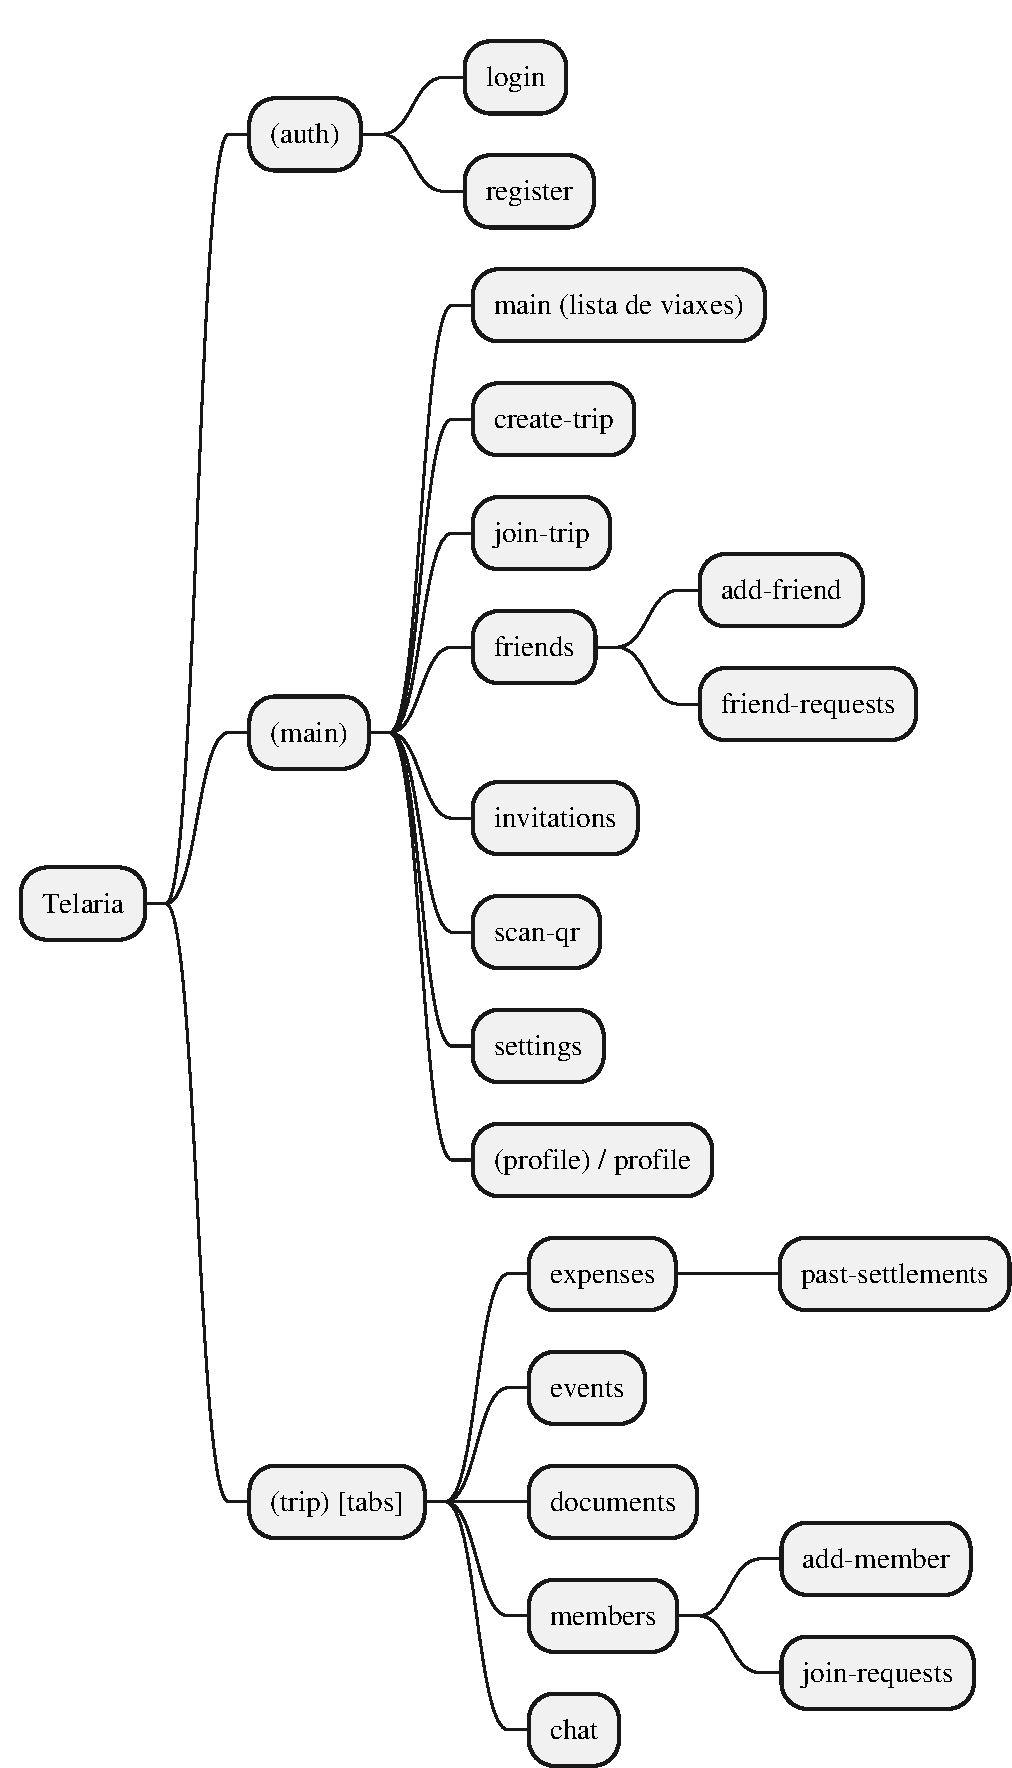
\includegraphics[width=0.55\textwidth]{diagrams/navegacion.pdf}
  \caption{Mapa de navegación da aplicación.}
  \label{fig:navegacion}
\end{figure}

\section{Deseño da interface de usuario}

Alén da súa arquitectura técnica, o frontend conta cunha linguaxe visual propia e coidada.
Nesta sección descríbese o sistema visual, os compoñentes e patróns de interface, as
animacións e a accesibilidade.

\subsection{Linguaxe visual e temas}

A identidade visual de Telaria articúlase arredor dunha paleta monocromática centrada no
violeta. A
aplicación ofrece dous temas (claro e escuro) que o usuario selecciona manualmente e que se
conservan entre sesións (non segue automaticamente o axuste do sistema). A
Figura~\ref{fig:paleta} recolle as cores principais.

\begin{figure}[H]
  \centering
  \renewcommand{\arraystretch}{1.3}
  \begin{tabular}{@{}ll@{}}
    \textbf{Globais}    & \swatch{telPrimary}{\#8b3ce0}\quad\swatch{telWarning}{\#dc2626}\\[6pt]
    \textbf{Tema claro} & \swatch{telLbg}{\#f7f3ff}\quad\swatch{telLui}{\#ede3fd}\quad\swatch{telLtext}{\#3d1e7a}\quad\swatch{telLtint}{\#7c3aed}\quad\swatch{telLborder}{\#d4c2f9}\\[6pt]
    \textbf{Tema escuro}& \swatch{telDbg}{\#07050f}\quad\swatch{telDui}{\#0e0b1f}\quad\swatch{telDtext}{\#e8e0fa}\quad\swatch{telDtint}{\#a855f7}\quad\swatch{telDborder}{\#2b1650}\\
  \end{tabular}
  \caption{Paleta de cores de Telaria: cores globais e específicas de cada tema.}
  \label{fig:paleta}
\end{figure}

A tipografía emprega as fontes do sistema (sen fontes propias) e a xerarquía visual
conséguese mediante o peso e o espazado entre letras, máis que mediante familias
tipográficas distintas. A estética compleméntase con esquinas redondeadas e brillos sutís
(\textit{glow}) de ton violeta arredor dos elementos destacados.

\subsection{Compoñentes e patróns de interface}

A interface constrúese sobre un conxunto de compoñentes reutilizables con tema:
\texttt{ThemedText}, \texttt{ThemedButton} e \texttt{ThemedInput} encapsulan o estilo base;
\texttt{UserAvatar} mostra a imaxe do usuario ou, na súa ausencia, as iniciais, e respecta o
modo de aforro de datos; e \texttt{SegmentedControl} ofrece un selector con animación. O
cromo de navegación componse dunha barra de pestanas inferior que resalta a pestana activa
cun brillo e amosa badges de notificación, e dun menú lateral que se presenta como panel
deslizante inferior (\textit{bottom sheet}). O asistente de IA ábrese nun modal a pantalla
completa accesible desde un botón flotante. Completan o repertorio as tarxetas, os modais e
os diálogos de confirmación. A Figura~\ref{fig:ui-pantalla} mostra unha pantalla representativa.

\begin{figure}[H]\centering
  
\includegraphics[width=0.45\textwidth]{calendar.jpeg}
  \caption{Pantalla representativa da aplicación (calendario compartido da viaxe).}\label{fig:ui-pantalla}
\end{figure}

\subsection{Animacións e retroalimentación visual}

As animacións baséanse na API \texttt{Animated} de React Native. A retroalimentación de
pulsación aplica unha lixeira redución de escala e de opacidade aos elementos interactivos;
o \texttt{SegmentedControl} desprázase cun efecto de resorte; o escáner de códigos QR mostra
unha liña de varrido e un pulso; o contido reaxústase de forma animada á altura do teclado; e
o fondo das pantallas inclúe unha textura sutil (grella de puntos e manchas de cor ambientais)
que achega profundidade sen distraer.

\subsection{Accesibilidade}

No tocante á accesibilidade, a aplicación adopta varias medidas, aínda que tamén deixa marxe
de mellora que se describe con transparencia.

\textbf{Medidas adoptadas.} A aplicación está internacionalizada en galego, castelán e inglés
(cf.\ RNF-US-02), o que mellora a comprensión para usuarios de distintas linguas. O dobre tema
claro/escuro axuda ás persoas sensibles á luz ou con baixa visión, e o modo de aforro de datos
reduce a carga de imaxes. Ademais, os controis interactivos de toda a aplicación, a barra de
pestanas (que expón a pestana seleccionada mediante \texttt{accessibilityState}), os menús, o
asistente de IA e os botóns de acción das distintas pantallas (engadir, eliminar, navegar,
etc.), incorporan etiquetas (\texttt{accessibilityLabel}) e roles (\texttt{accessibilityRole})
de accesibilidade internacionalizados, de xeito que os lectores de pantalla anuncian cada
control co seu nome; a retroalimentación de pulsación é consistente en toda a interface.
Finalmente, a paleta de cores axustouse para que as combinacións de texto e fondo cumpran o
limiar de contraste \mbox{WCAG~AA}. Ademais, respéctase a preferencia de movemento reducido do
sistema (as animacións desactívanse ou acúrtanse cando o usuario a activa) e as compoñentes de
texto compartidas limitan o factor máximo de escala da tipografía
(\texttt{maxFontSizeMultiplier}) para que os tamaños grandes non rompan os deseños. Os controis
interactivos amplían ademais a súa área de pulsación (\texttt{hitSlop}) ata o tamaño mínimo
recomendado, e as accións consecuentes (saír da viaxe, eliminar a conta, pechar a sesión, etc.)
inclúen pistas (\texttt{accessibilityHint}) que describen o seu efecto.

\textbf{Limitacións.} O límite de escala da tipografía aplícase ás compoñentes de texto
compartidas e aos controis principais, pero aínda non a todos os textos da interface.

\textbf{Traballo futuro.} Unha mellora adicional incluiría estender o límite de escala da
tipografía a todos os textos da interface (e non só ás compoñentes compartidas). Esta revisión
pode apoiarse nas
comprobacións de accesibilidade da ferramenta react-doctor, xa presente no proxecto. A
Figura~\ref{fig:ui-temas} ilustra os dous temas.

\begin{figure}[H]
  \centering
  \subcaptionbox{Tema claro\label{fig:ui-temas-light}}{%
    
\includegraphics[height=11cm]{balances-light.jpeg}}
  \hspace{0.8cm}
  \subcaptionbox{Tema escuro\label{fig:ui-temas-dark}}{%
    
\includegraphics[height=11cm]{balances-dark.jpeg}}
  \caption{Comparación dos temas claro e escuro: pantalla de balances da viaxe.}
  \label{fig:ui-temas}
\end{figure}

\subsection{Análise heurística}

Co obxectivo de identificar posibles problemas de usabilidade desde unha perspectiva
experta, a interface de Telaria avaliouse segundo as \textbf{dez heurísticas de
usabilidade de Nielsen}~\cite{nielsen1994usability}. Esta avaliación complementa as
probas de pensamento en voz alta con usuarios reais descritas no
capítulo~\ref{ch:probas}. A Táboa~\ref{tab:heuristicas} resume como o deseño aborda
cada heurística.

\begin{table}[H]
  \centering
  \begin{tabularx}{\textwidth}{@{}lX@{}}
    \toprule
    \textbf{Heurística} & \textbf{Aplicación en Telaria} \\
    \midrule
    Visibilidade do estado do sistema &
      Indicadores de carga nas chamadas á API, progresión visual na subida de
      documentos, actualizacións en tempo real do chat e do asistente de IA
      (\textit{streaming}) e \textit{badges} de notificación na barra de pestanas. \\
    \addlinespace
    Correspondencia co mundo real &
      Terminoloxía de viaxes familiar (gastos, membros, eventos, calendario),
      categorías de gasto naturais e mapa interactivo para seleccionar localizacións. \\
    \addlinespace
    Control e liberdade do usuario &
      Navegación cara atrás en todos os niveis, posibilidade de abandonar unha viaxe
      e de eliminar a conta, e cancelación de calquera modal sen consecuencias. \\
    \addlinespace
    Consistencia e estándares &
      Compoñentes con tema reutilizables (\texttt{ThemedText}, \texttt{ThemedButton},
      \texttt{ThemedInput}), paleta e tipoloxía uniformes e patróns de navegación
      estándar para plataformas móbiles (barra de pestanas, \textit{bottom sheet}). \\
    \addlinespace
    Prevención de erros &
      Validación de formularios antes do envío, diálogos de confirmación para
      operacións destrutivas (eliminar conta, saír da viaxe) e tipado estrito de
      extremo a extremo a través do contrato OpenAPI. \\
    \addlinespace
    Recoñecemento antes que recordo &
      Barra de pestanas sempre visible, historial de mensaxes e de gastos accesible
      en todo momento e información contextual da viaxe activa presente en cada
      pantalla. \\
    \addlinespace
    Flexibilidade e eficiencia &
      Unión a viaxes por código QR, convites directos a amigos e acceso inmediato
      aos documentos do día seleccionado no calendario. \\
    \addlinespace
    Deseño estético e minimalista &
      Estética limpa, ausencia de información superflua en
      pantalla e textura de fondo sutil que non distrae do contido principal. \\
    \addlinespace
    Axuda para recuperarse de erros &
      Mensaxes de erro claras nas operacións fallidas, formato \textit{Problem
      Details} (RFC~7807)~\cite{rfc7807} nas respostas de erro da API e
      retroalimentación visual ante fallos de rede. \\
    \addlinespace
    Axuda e documentación &
      Asistente de IA integrado que coñece o contexto da viaxe activa (eventos,
      gastos e historial de chat) e pode responder consultas do usuario en
      linguaxe natural. \\
    \bottomrule
  \end{tabularx}
  \caption{Avaliación heurística da interface de Telaria segundo as dez heurísticas de Nielsen.}
  \label{tab:heuristicas}
\end{table}

\section{Fluxos de comunicación entre compoñentes}

\subsection{Autenticación e renovación de tokens}

O inicio de sesión devolve un \textit{access token} JWT de vida curta e un
\textit{refresh token} opaco. Cando o \textit{access token} caduca, o cliente detéctao
ante unha resposta \texttt{401} e renóvao de forma transparente, sen requirir unha nova
autenticación do usuario (Figura~\ref{fig:seq-auth}).

\begin{figure}[H]
  \centering
  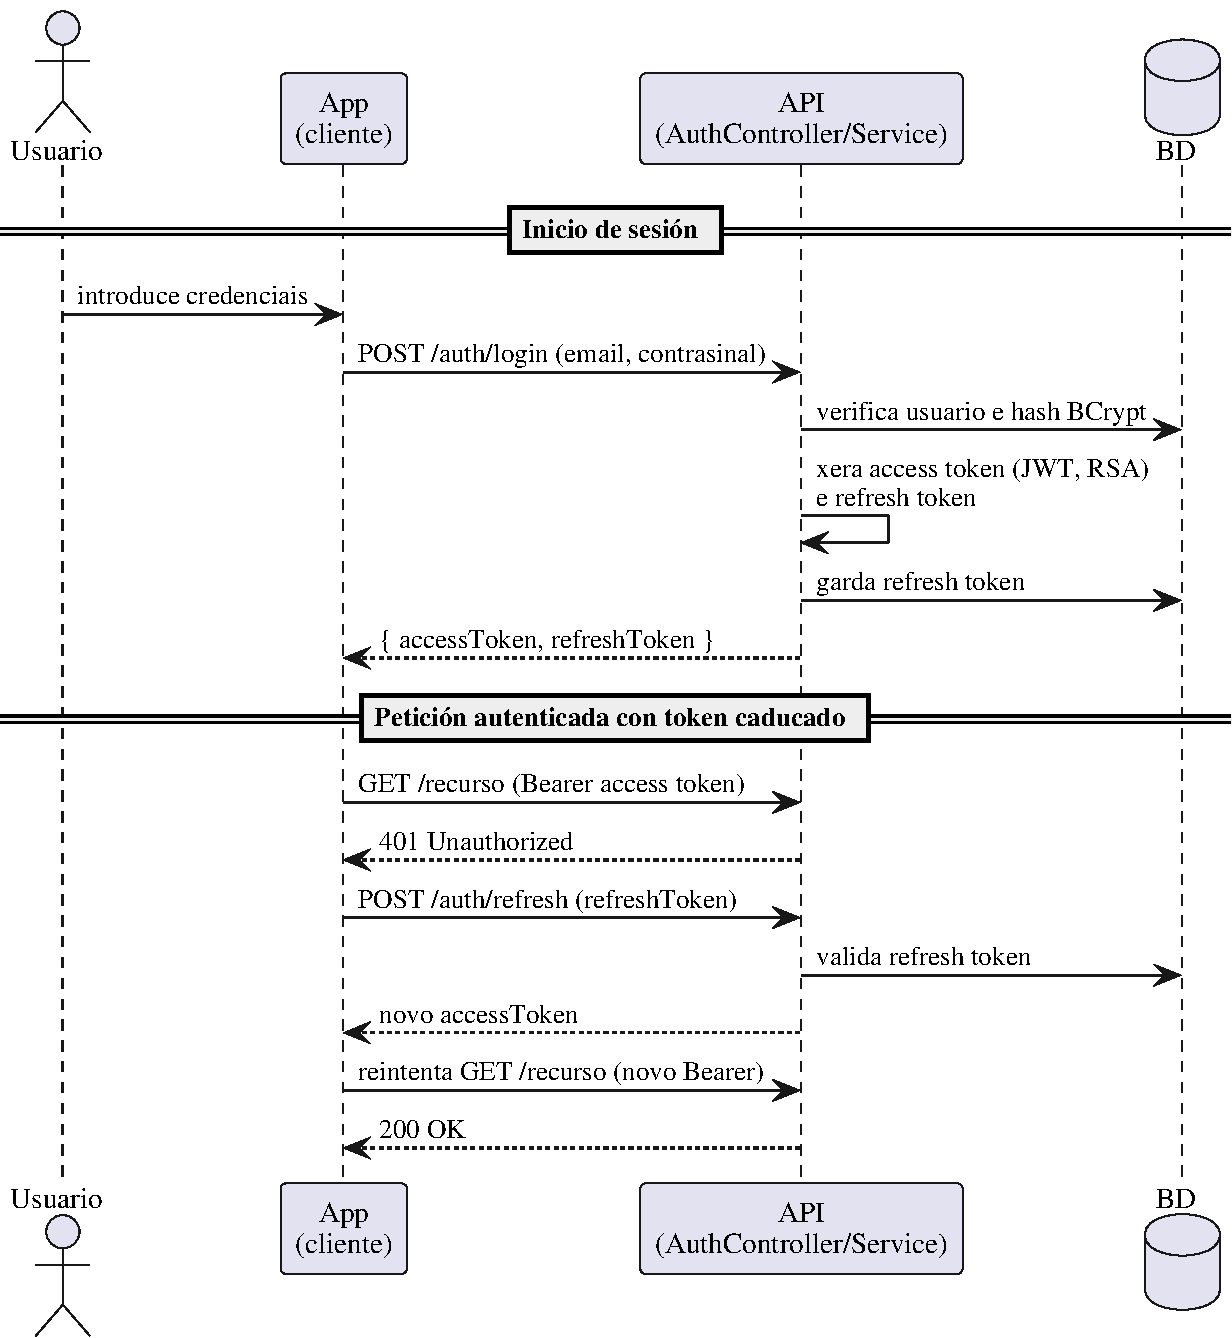
\includegraphics[width=0.7\textwidth]{diagrams/seq-auth.pdf}
  \caption{Secuencia de autenticación e renovación do \textit{access token}.}
  \label{fig:seq-auth}
\end{figure}

\subsection{Chat de grupo en tempo real (SSE)}

Cando un membro abre o chat, o cliente subscríbese a un fluxo SSE. Ao enviar outro membro
unha mensaxe, o servidor persístea e difúndea de inmediato a todos os subscritores
conectados (Figura~\ref{fig:seq-chat}).

\begin{figure}[H]
  \centering
  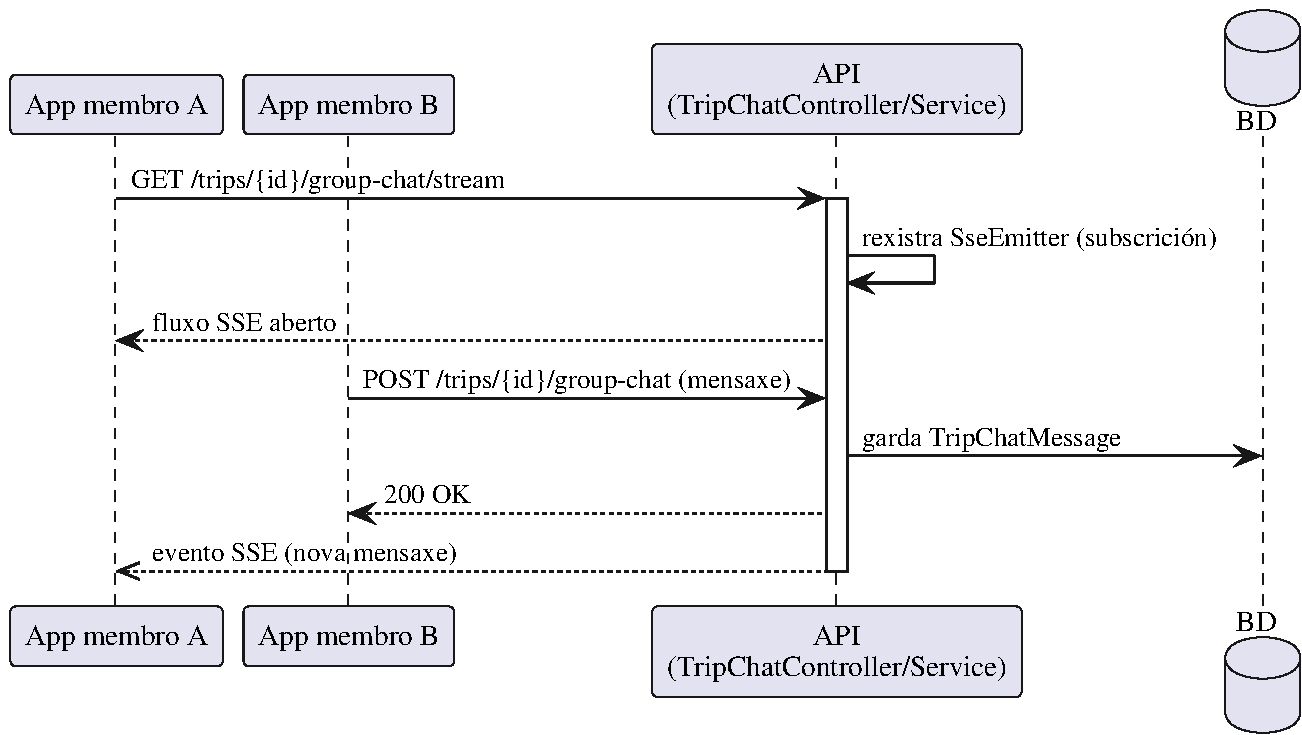
\includegraphics[width=0.8\textwidth]{diagrams/seq-chat-sse.pdf}
  \caption{Secuencia do chat de grupo mediante \textit{Server-Sent Events}.}
  \label{fig:seq-chat}
\end{figure}

\subsection{Subida de documentos con URL prefirmada}

A subida realízase en varios pasos para que o ficheiro non atravese o backend: este crea
o rexistro e devolve unha URL prefirmada, o cliente sobe o ficheiro directamente ao
almacén e, finalmente, confirma a subida; se o ficheiro é unha imaxe, xérase unha
miniatura de forma asíncrona (Figura~\ref{fig:seq-upload}).

\begin{figure}[H]
  \centering
  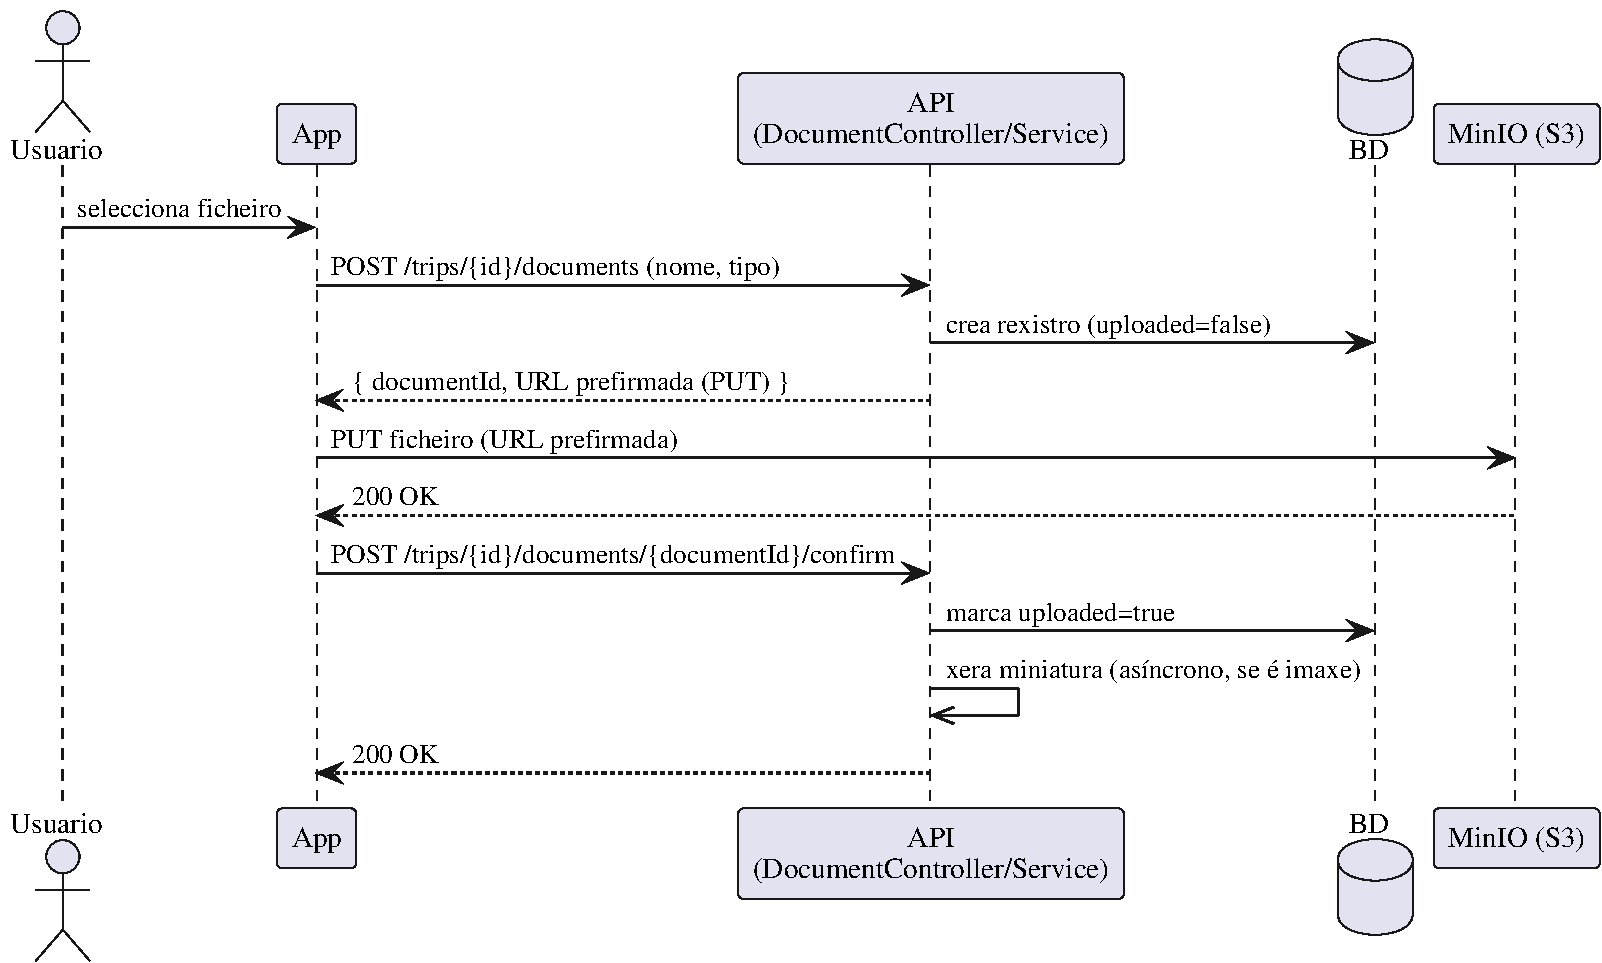
\includegraphics[width=0.9\textwidth]{diagrams/seq-upload.pdf}
  \caption{Secuencia de subida de documentos con URL prefirmada.}
  \label{fig:seq-upload}
\end{figure}

\subsection{Asistente de IA en \textit{streaming}}

Ao recibir unha consulta, o servidor constrúe o contexto da conversa a partir dos
eventos e gastos da viaxe e das últimas mensaxes, e remítello ao modelo local (Ollama). A
resposta devólvese token a token cara ao cliente mediante SSE, ofrecendo unha experiencia
de escritura progresiva (Figura~\ref{fig:seq-ia}).

\begin{figure}[H]
  \centering
  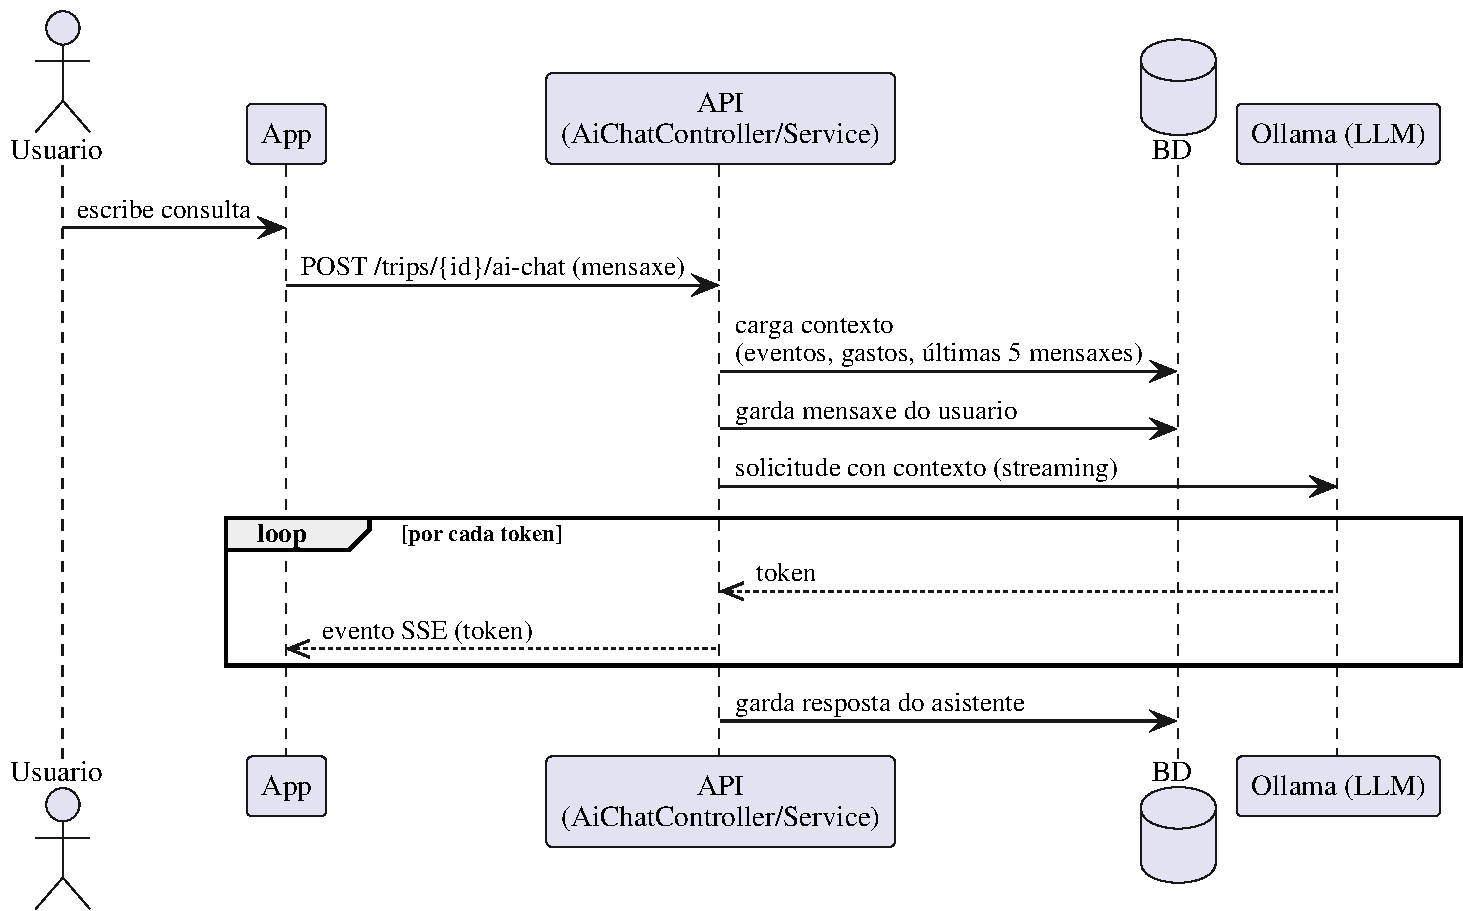
\includegraphics[width=0.85\textwidth]{diagrams/seq-ia.pdf}
  \caption{Secuencia do asistente de IA con resposta en \textit{streaming}.}
  \label{fig:seq-ia}
\end{figure}

\section{Seguridade}

A seguridade do sistema descansa sobre os seguintes piares de deseño:

\begin{itemize}
  \item \textbf{Autenticación con JWT asinado.} No inicio de sesión, o backend asina os
        seus propios \textit{access tokens} (JWT) cunha clave privada RSA almacenada nun
        \textit{keystore}; en cada petición valida a sinatura do token coa clave pública,
        sen necesidade de consultar a base de datos. Esta validación de tokens portadores
        (\textit{bearer}) apóiase no soporte de JWT de Spring Security~\cite{springsecurity}.
        Non se implementa o protocolo OAuth~2.0: non existe un servidor de autorización
        externo nin fluxos de delegación, senón un esquema de autenticación propio baseado
        en tokens autoasinados.
  \item \textbf{Sesións sen estado.} O servidor non mantén sesión; cada petición é
        autosuficiente grazas ao token, o que mellora a escalabilidade.
  \item \textbf{Contrasinais protexidos.} Os contrasinais almacénanse cifrados con
        BCrypt~\cite{bcrypt}.
  \item \textbf{Autorización por pertenza.} O acceso aos recursos dunha viaxe está
        condicionado a que o usuario sexa membro dela.
  \item \textbf{Confirmación en operacións sensibles.} O cambio de correo electrónico e a
        eliminación de conta requiren reintroducir o contrasinal actual.
\end{itemize}

\section{Integración con servizos externos}

\begin{itemize}
  \item \textbf{Ollama.} O asistente de IA delega a inferencia nun modelo de linguaxe
        executado localmente, ao que o backend accede por HTTP en modo \textit{streaming}.
  \item \textbf{Almacén de obxectos (MinIO/S3).} A xestión de ficheiros realízase co AWS
        SDK; o backend nunca recibe nin serve os ficheiros, senón que xera URLs
        prefirmadas de subida e descarga cunha validez limitada.
  \item \textbf{Procesamento de imaxes.} As miniaturas de previsualización e o
        redimensionamento de avatares prodúcense reducindo a imaxe a un tamaño máximo e
        convertíndoa a JPEG, sempre fóra da ruta de petición.
\end{itemize}

\section{Equipamento hardware e software}

O desenvolvemento e a execución do sistema requiren o seguinte equipamento, resumido na
Táboa~\ref{tab:equipamento}. Dado que ningunha destas tecnoloxías constituía un requisito
previo, a súa elección xustifícase nas seccións anteriores e na introdución.

\begin{table}[H]
  \centering
  \begin{tabularx}{\textwidth}{@{}lX@{}}
    \toprule
    \textbf{Ámbito} & \textbf{Tecnoloxías e ferramentas} \\
    \midrule
    Frontend        & React Native, Expo, TypeScript, React Query; ferramentas de Node.js. \\
    Backend         & Java, Spring Boot, Spring Data JPA, Spring Security; construción con Gradle. \\
    Persistencia    & PostgreSQL. \\
    Almacenamento   & MinIO (compatible con S3). \\
    Intelixencia artificial & Ollama (modelo de linguaxe local). \\
    Despregamento   & Contedores OCI xestionados con Podman. \\
    Cliente final   & Dispositivo móbil iOS ou Android con conexión á rede. \\
    \bottomrule
  \end{tabularx}
  \caption{Equipamento software e hardware do sistema.}
  \label{tab:equipamento}
\end{table}
